\section{Counting and Probability}

\subsection{Counting}

\begin{description}
  \item[C.1-1] {\itshape How many $k$-substrings does an $n$-string have? (Consider identical $k$-substrings at different positions to be different.) How many substrings does an $n$-string have in total?}
    \begin{ex}
      Il y a $S_k = n - k + 1$ $k$-sous-cha\^ines dans une $n$-cha\^ine. Le nombre total de sous-cha\^ines dans une $n$-cha\^ine est donc \[\sum_{k=1}^n S_k = \frac{n(n+1)}{2}.\]
    \end{ex}
  \item[C.1-2] {\itshape An $n$-input, $m$-output boolean function is a function from  $\{\textrm{TRUE}, \textrm{FALSE}\}^n$ to $\{\textrm{TRUE}, \textrm{FALSE}\}^m$. How many $n$-input, $1$-output boolean functions are there? How many $n$-input, $m$-output boolean functions are there?}
    \begin{ex}
      Le cardinal de l'ensemble de fonction de $E$ dans $F$  est $|F|^{|E|}$. Particuli\`erement pour les fonctions bool\'eenes, on a :
      \begin{itemize}
        \item pour $E = \{\textrm{TRUE}, \textrm{FALSE}\}^n$ et $F=\{\textrm{TRUE}, \textrm{FALSE}\}$, $|F|^{|E|} = 2^{2^n}$ ;
        \item pour $E = \{\textrm{TRUE}, \textrm{FALSE}\}^n$ et $F=\{\textrm{TRUE}, \textrm{FALSE}\}^m$, $|F|^{|E|} = {(2^m)}^{2^n}$.
      \end{itemize}
    \end{ex}
  \item[C.1-3] {\itshape In how many ways can $n$ professors sit around a circular conference table? Consider two seatings to be the same if one can be rotated to form the other.}

    \begin{ex}
      On consid\`ere tout d'abord le cas de si\`eges rang\'es lin\'eairement. Dans ce cas, on a $n!$ arrangements. Dans le cas circulaire, on peut d\'efinir une relation d'\'equivalence $\mathcal{R}$ qui regroupe les arrangements qui peuvent \^etre obtenus par une permutation circulaire. De ce fait, il y a exactement $n$ \'el\'ements dans chaque classe. Le nombre d'arrangement de si\`eges plac\'es circulairement est en fait le cardinal de l'espace quotient\'e par $\mathcal{R}$. Donc il y a $\frac{n!}{n} = (n-1)!$ arrangements.
    \end{ex}

  \item[C.1-4] {\itshape In how many ways can we choose three distinct numbers from the set $\{1, 2,\ldots, 99\}$ so that their sum is even?}
    \begin{ex}
      Pour obtenir un nombre pair en sommant trois nombres distincts de l'ensemble $E = \{1, 2, \ldots, 99\}$, il y a deux possibilit\'es :
      \begin{itemize}
        \item pair + pair + pair = pair ;
        \item impair + impair + pair = pair .
      \end{itemize}
      Dans l'ensemble $E$, il y a $50$ nombres impairs et $49$ nombres pairs. Finalement, le nombre de combinaisons est :
      \[ \binom{49}{3} + \binom{50}{2}\binom{49}{1} = 78449.  \]
      
    \end{ex}
  \item[C.1-5] {\itshape Prove the identity \[\binom{n}{k} = \frac{n}{k}\binom{n-1}{k-1}\] for $ 0 < k \le n$.}

    \begin{ex}
      \[ \binom{n}{k} = \frac{n!}{k!(n-k)!} = \frac{n\cdot(n-1)!}{k(k-1)!((n-1)-(k-1))!} = \frac{n}{k}\binom{n-1}{k-1}.\]
    \end{ex}

  \item[C.1-6] {\itshape Prove the identity \[\binom{n}{k} = \frac{n}{n-k}\binom{n-1}{k}\] for $ 0 \le k < n$.}
    \begin{ex}
      \[ \binom{n}{k} = \frac{n}{n-k}\cdot\frac{(n-1)!}{k!((n-1)-k)!} = \binom{n-1}{k}.\]
    \end{ex}
  \item[C.1-7] {\itshape To choose $k$ objects from $n$, you can make one of the objects distinguished and consider whether the distinguished object is chosen. Use this approach to prove that \[\binom{n}{k} = \binom{n-1}{k}+\binom{n-1}{k-1}.\]}
    \begin{ex}\mbox{}\\ %TODO: fix diagram
      {
        \begin{figure}[H]
          \centering
        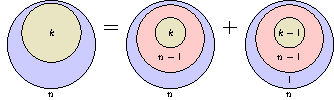
\includegraphics[scale=1.5]{img/C_1-7/C_1-7.pdf}
        \caption{\frquote{combinaison de $k$ parmi $n$}}
          \label{fig:C.1-7}
        \end{figure}
      }
      On fixe un \'el\'ement parmi les $n$ et on en choisit $k$. Si l'\'el\'ement est choisi, il y a $\binom{n-1}{k-1}$ moyens de choisir les autres; sinon les $k$ \'el\'ements choisis sont inclus dans les $n-1$ restants et il y a $\binom{n-1}{k}$ moyens de choisir.
    Conclusion : $ \binom{n}{k} = \binom{n-1}{k}+\binom{n-1}{k-1}$, d'o\`u ce que montre la figure (\ref{fig:C.1-7}).     
    \end{ex}
  \item[C.1-8] {\itshape Using the result of Exercise C.1-7, make a table for $n = 0, 1, \ldots, 6$ and $ 0\le k \le n$ of the binomial coefficients $\binom{n}{k}$ with $\binom{0}{0}$ at the top, $\binom{1}{0}$ and $\binom{1}{1}$ on the next line, and so forth. Such a table of binomial coefficients is called \textbf{Pascal’s triangle}.}
    \begin{ex}\mbox{}
      \begin{figure}[H]
        \centering
        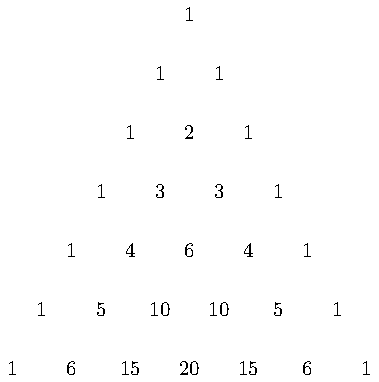
\includegraphics{img/C_1-8/C_1-8.pdf}
        \caption{Triangle de Pascal}
        \label{fig:}
      \end{figure}
    \end{ex}
  \item[C.1-9] {\itshape Prove that \[ \sum_{i=1}^n i = \binom{n+1}{2}.\]}
    \begin{ex}
      \[\sum_{i=1}^ni = \frac{n(n+1)}{2} = \frac{(n+1)!}{(n-2)!2!} = \binom{n+1}{2}.\]
    \end{ex}
  \item[C.1-10] {\itshape Show that for any integers $n \ge 0$ and $ 0\le k \le n$, the expression $\binom{n}{k}$ achives its maximum value when $k = \lfloor n/2 \rfloor$ or $k = \lceil n/2 \rceil$.}
    \begin{ex}
      Il y a deux points de vue :
      \begin{enumerate}
        \item la sym\'etrie : $\binom{n}{k} = \binom{n}{n-k}$ ;
        \item la croissance :
        Comparons $\binom{n}{k}$ et $\binom{n}{k+1}$ : 
        \begin{align*}
          \binom{n}{k} < \binom{n}{k+1} &\iff \frac{n!}{k!(n-k)!} < \frac{n!}{(k+1)!(n-k-1)!}\\
          &\iff k!(n-k)! > (k+1)!(n-k-1)!\\
          &\iff (n-k)! > (k+1)(n-k-1)!\\
          &\iff n-k>k+1\\
          &\iff n > 2k+1\\
          &\iff k<\frac{n-1}{2}.
        \end{align*}
      \end{enumerate}
      En r\'eunissant ces deux r\'esultats, \`a $n$ fix\'e, on observe que les coefficients $\binom{n}{k}$ pour $k = 0, \ldots, \lfloor \frac{n}{2} \rfloor$ croissent et atteignent une valeur maximale lorsque $k = \lfloor n/2 \rfloor$ et $ k = \lceil n/2 \rceil$ (par sym\'etrie).
    \end{ex}

  \item[C.1-11 $\star$] {\itshape }
  \item[C.1-12 $\star$] {\itshape }
  \item[C.1-13 $\star$] {\itshape }
  \item[C.1-14 $\star$] {\itshape }
  \item[C.1-15 $\star$] {\itshape }
\end{description}
